\section{Memory Efficient Convolutions}
\begin{figure}
	\centering
	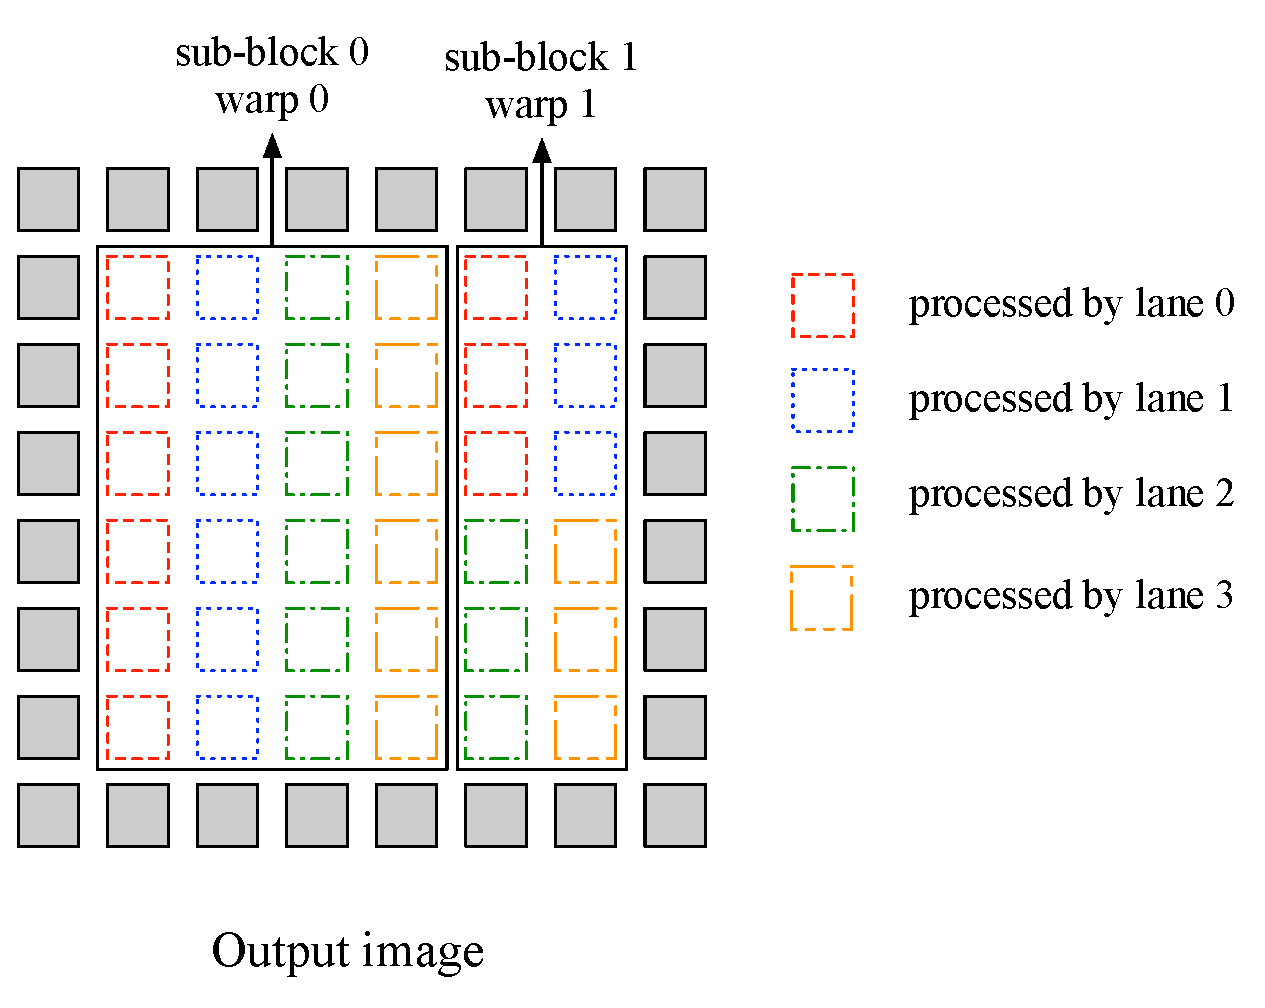
\includegraphics[width=0.9\columnwidth,height=5.5cm]{./figure/overalldesign.eps}
\caption{The output is produced by sliding a $3 \times 3$ filter over an $8 \times 8$ input with one pad. Edge elements and inner elements are processed by different thread blocks. We assume that the warp size is 4 and thus having $laneid=threadid\%4$.}
\label{fig:overalldesign}
\end{figure}


This section demonstrates the implementation of the two proposed reuse algorithms on 2D and 3D convolutions. The main difference between the
implementations in the 2D and 3D convolutions lies in the loading of filters. For the former, we focus on the scenario where a filter is used to
slide over a large image. Therefore, we can load the entire filter into a shared memory, and only one thread block needs to load the
filter once. For the latter, we focus on the scenario where many filters are used to slide over a batch of images, which are often the
first layers of CNNs. All filters cannot fit into the shared memory; hence, we need to load the filters multiple times.

To simplify the discussion, we use a 2D convolution running at an NVIDIA GPU as an example. We first divide the output
into sub-blocks, which contain exactly 32 (warp size) columns each, except for the last sub-block, which may contain less than 32 columns.
Each thread block processes one or more sub-blocks, and each warp processes one sub-block. The threads within the same warp process the adjacent columns of one sub-block.
\begin{algorithm}
	\KwIn{$I$, $F$, $O$, $subBlockHeight$}
	\KwOut{$O$}
	load filter into shared memory\;
	$\_\_syncthreads()$\;
	\If{$blockIdx.x \textless gridDim.x-1$}{
		Calculate the index of the first input element this thread needs, denoted as $baseIndex$\;
		\For{$i \gets 0$ \KwTo $I_C$}{
			$inputIndex \gets baseIndex+i*I_H*I_W$\;
			\For{$j \gets 0$ \KwTo $subBlockHeight$}{
				Use Algorithm \ref{algo:basic} and Algorithm \ref{algo:basic2} to load input elements the thread needs, the loaded elements are denoted as $row$\;
				
				Use Algorithm \ref{algo:rowreuse} to calculate output elements and store results into thread local register array $sum$\;
			}
		}
		Write array $sum$ into global memory\;
	}
	\Else{
		Process the remaining inner elements of $O$\;
		Process the edge elements of $O$\;
	}
	\caption{Overall design}
	\label{algo:overalldesign}
\end{algorithm}

Figure \ref{fig:overalldesign} shows the mapping process of the threads onto the output elements. Given that 2D convolutions normally produce an output image that has the same size as the input image, the latter should be padded. But we do not actually allocate memory on the GPU. We use different methods to calculate the edge and inner elements of the output image. The edge and inner elements are represented by the shaded and dashed squares in Figure \ref{fig:overalldesign}, respectively.

We also demonstrate how to deal with the inner elements and how to  calculate the edge elements using the same method for the inner elements. Each warp is assumed to contain four threads (Figure \ref{fig:overalldesign}). The inner elements are divided into two
sub-blocks. Sub-block 0 contains four columns, which represent the warp size, whereas sub-block 1 contains only two columns. To utilize the threads within a warp, we divide the last two columns evenly among the four threads. A generalized overall design is shown in Algorithm \ref{algo:overalldesign}.

In the first two lines of Algorithm \ref{algo:overalldesign}, we first load the filter into the shared memory. Then, we process the sub-blocks with exactly 32 columns and the last sub-block in Lines 3-13 and 14-17, respectively. Each thread calculates one column of the output elements. First, each thread calculates the address of the first input element it needs (Lines 4-6). Second, each thread uses Algorithms \ref{algo:basic} and \ref{algo:basic2} to fulfill the vector $row$, which contains a row of the sub-block (Line 8). Third, each thread passes the
vector $row$ to Algorithm \ref{algo:rowreuse} to calculate multiple output elements and store results in register array $sum$ (Line 9).
Lastly, each thread writes the result array $sum$ into the global memory (Line 12).
